\chapter{Complessità del Calcolo}
  Nei capitoli precedenti si è dimostrato come esistano alcuni problemi che, pur essendo ben definiti, non sono risolvibili algoritmicamente, per cui non esiste una TM in grado di risolvere quel determinato problema. Un'altra difficoltà da tenere in considerazione quando si manipolano i problemi, risiede nel tempo di esecuzione, ovvero il tempo impiegato dal programma per fornire una soluzione: se non è possibile ottenere una soluzione in un tempo ragionevole, ovviamente, il problema diventa intrattabile, nonostante sia teoricamente risolvibile.

  Il concetto di intrattabilità è strettamente correlato al concetto di complessità del calcolo: più il problema è complesso e meno questo diventa trattabile. Informalmente, la complessità indica una misura del prezzo da pagare per risolvere il problema. Le risorse che si utilizzano per la risoluzione di un problema sono principalmente due: lo spazio, ovvero la memoria necessaria all'algoritmo, e il tempo richiesto per produrre la soluzione. Si parlerà quindi di complessità spaziale e di complessità temporale.

  Si osservi inoltre che le due risorse, quella temporale e quella spaziale, seppur sembrino indipendenti l'una dall'altra, sono in realtà correlate: alla riduzione di utilizzo di una risorsa aumenta l'altra e viceversa. 

  \section{Analisi di complessità}
  La complessità del calcolo dipende dalla dimensione e, spesso, anche dai particolari valori assunti dai dati in ingresso. Per questo motivo, si rende necessario effettuare un'analisi del caso pessimo, del caso medio e del caso ottimo, in funzione della dimensione dei dati in ingresso. Più formalmente, tali casi rappresentano rispettivamente la scelta di ingressi per cui viene eseguito il massimo numero di istruzioni nel programma, il comportamento del programma in relazione alla possibile distribuzione dei dati e la scelta di input per cui viene eseguito il minor numero di istruzioni.

  In generale, il caso ottimo non è di particolare interesse e il caso medio richiede la conoscenza della distribuzione dei dati in ingresso (non sempre nota). Il caso pessimo, invece, è particolarmente interessante in quanto fornisce i peggiori risultati ottenibili dall'algoritmo in termini di consumo di spazio o tempo; si garantisce quindi che tutte le soluzioni proposte dall'algoritmo abbiano un dispendio di risorse minore rispetto al caso pessimo, indipendentemente dalla tipologia degli ingressi. Dunque, se il caso pessimo è ritenuto accettabile, allora anche tutti gli altri casi lo sono. 

  Inoltre, a differenza di quanto analizzato per la risolvibilità dei problemi, la complessità non è collegata solo al problema che si vuole affrontare, ma dipende anche dell'algoritmo che si utilizza per risolverlo. 

  \paragraph{}
  Nel capitolo sugli automi, è stato più volte affermato che le Macchine di Turing sono il formalismo più potente che si ha a disposizione per la risoluzione di prblemi, dunque, risulta ragionevole definire la complessità temporale e spaziale impiegando un tale modello.

  \begin{definition} \label{complessita temporale} 
    Sia \(M\) una TM deterministica a \(k\) nastri e sia \(x\in I^*\). Sia \(c_0\vdash c_1\vdash....\vdash c_r\) una computazione, ovvero una sequenza di transizioni di \(M\) tale che \(c_0=<q_0,\;\!\uparrow\! x,\; \!\uparrow\! Z_0,\; ...,\; \!\uparrow\! Z_0>\) e \\ \(c_i=<q_i,\;x_i\!\uparrow\! y_i,\; \alpha_{i1}\!\uparrow\! \beta_{i1},\; ...,\; \alpha_{ik}\!\uparrow\! \beta_{ik}>\), in cui \(c_r\) è una configurazione di arresto, se esiste. Allora, la funzione che rappresenta la complessità temporale \({T}_M\) di \(M\) è definita nel seguente modo:
    \begin{equation*}
      {T}_M=if\;la\;computazione\;termina\;then\;r\;else\;\infty.
    \end{equation*}
  \end{definition}

  Informalmente, quindi, la complessità temporale viene definita come una funzione che fornisce il numero esatto di passi richiesti da una TM per raggiungere la propria configurazione di arresto, se esiste, a partire dalla configurazione iniziale, per una qualsiasi stringa in ingresso. analogamente, si può definire la complessità spaziale come una funzione che fornisce il numero massimo di celle del nastro utilizzate.

  \begin{definition} \label{complessita spaziale}
    Siano M, x, \(c_0,...,c_r\) definiti come nella definizione \ref{complessita temporale}. La funzione che rappresenta la complessità spaziale \({S}_M\) di M è definita nel seguente modo:

    \begin{equation*}
      \displaystyle {S}_M=\sum_{j=1}^{k} max_{i\in\{0,1,...,r\}}(|\alpha_{ij}|)
    \end{equation*}
    Inoltre, vale che:
    \begin{equation*}
      \forall x, \frac{{S}_M}{k}\le {T}_M(x)
    \end{equation*}
  \end{definition}

  Si noti, inoltre, che la definizione di \({S}_M(x)\) prende in considerazione solamente i nastri di memoria e ignora sia il nastro di ingresso che il nastro di uscita per il calcolo della complessità.

  Secondo le definizioni \ref{complessita temporale} e \ref{complessita spaziale}, sia \({T}_M\) che \({S}_M\) sono funzioni definite su \(I^*\), ma nella pratica la complessità di una soluzione dipende sia dal contenuto dell'ingresso che dalla sua dimensione: a partire da questa osservazione, si erano introdotti i concetti di complessità nel caso pessimo, medio e ottimo, che si possono ridefinire nel seguente modo, alla luce delle definizioni appena date:

  \begin{definition}
    Il caso pessimo, ottimo e medio sono così definiti:
    \begin{itemize}
      \item Caso pessimo: \({T}_M(n)=max_{|x|=n}{T}_M(x)\);
      \item Caso ottimo: \({T}_M(n)=min_{|x|=n}{T}_M(x)\);
      \item Caso medio: \(\displaystyle {T}_M(n)=\frac{\sum_{|x|=n}{T}_M(x)}{|I|^n}\)
    \end{itemize}
  \end{definition}

  Una volta analizzata la complessità temporale tramite il formalismo delle macchine di Turing, si sposta l'attenzione sugli altri formalismi analizzati nel capitolo riguardante gli automi, in particolare sugli automi a stati finiti, sugli automi a pila e sulle macchine di turine a singolo nastro.

  \paragraph{}
  Dato un automa a stati finiti \(A\), si definisce la complessità temporale \({T}_A\) come l'intero \(i\) tale che \(\delta^i(q_0,x)=q\) per qualche \(q\), se esiste, ovvero il numero di transizioni effettuate per processare la stringa in ingresso \(x\) a partire dallo stato iniziale. Se \(\delta^*(q_0,x)\) è indefinita, si pone \({T}_A= |x|\), ovvero pari alla lunghezza della stringa in ingresso. \({T}_A\), evidentemente, indica il numero di mosse compiute da \(A\) durante il riconoscimento della stringa \(x\). Dunque, per ogni automa a stati finiti la complessità temporale \({T}_A\) cresce in maniera lineare con il crescere della lunghezza della stringa. Al contrario, la sua complessità spaziale \({S}_A\) non varia mai, in quanto gli FSA sono composti da un numero finito di stati definiti a priori, indipendentemente dalla lunghezza della stringa letta. 

  \paragraph{}
  Dato un automa a pila \(A\), si può analizzare sia la complessità temporale in funzione della stringa in ingresso (\({T}_A(x)\)), sia in funzione della lunghezza della stringa (\({T}_A(n)\)). Come per gli automi a stati finiti, quando si calcola la complessità temporale in funzione della stringa in ingresso, si contano il numero di passi che portano da una configurazione iniziale ad una configurazione finale. Quando invece si vuole utilizzare come parametro la lunghezza della stringa, la complessità temporale è calcolata come il massimo di tutte le complessità temporali in funzione delle stringhe in ingresso della lunghezza considerata. La complessità spaziale \({S}_A\), invece, viene associata al numero di celle di memoria della pila che vengono occupate dall'automa per portare a termine la computazione.

  \vspace*{10px}

  La complessità temporale e spaziale per le macchine di Turing a nastro singolo sono definite esattamente come per le TM a \(k\)-nastri. Data una macchina di Turing \(M\) a singolo nastro, la complessità spaziale \({S}_M(x)\), che corrisponde al massimo numero di celle del nastro di memoria occupate da \(M\) durante la computazione a fronte della stringa in ingresso \(x\), non può mai essere minore di \(|x|\), in quanto l'unico nastro presente in \(M\) è sia di ingresso, che di memoria, che di uscita. Ciò significa che l'unico nastro presente, di cui si deve analizzare l'occupazione, è precaricato con la stringa di ingresso \(x\). Per quanto riguarda la complessità spaziale, le TM a singolo nastro sono meno efficienti delle TM multinastro e, in alcuni casi, di altri formalismi analizzati. 
  
  In generale, le macchine di Turing multinastro sono il formalismo più potente ed efficiente per la computazione di problemi.


  \section{Comportamento asintotico}
  Nella maggior parte dei casi si analizza la complessità spaziale o temporale di un determinato algoritmo per valori molto grandi dell'ingresso \(x\), ovvero per \(x\) che tende ad infinito. In questi casi si analizza il comportamento asintotico dell'algoritmo, che fornisce un'approssimazione abbastanza precisa sul dispendio di risorse. La notazione dell'ordine di grandezza di una funzione, nota sotto il nome di notazione theta-grande (\(\Theta \)), sottolinea i fattori dominanti che influeanzano la creascita della sua complessità in funzione della dimensione dell'ingresso. Oltre alla notazione theta-grande, esistono anche le notazioni o-grande (O) e omega-grande (\(\Omega \)), le cui definizioni sono riportate di seguito:

  \begin{definition}[Notazione O]
    Siano \(g:\mathbb{N}\to\mathbb{R}^+\) ed \(f:\mathbb{N}\to\mathbb{R}^+\) due funzioni. La funzione g è in O(f) se e solo se esistono due numeri positivi c ed \(n_0\) tali che per ogni \(n\ge n_0,\; g(n)\le cf(n)\). Ciò significa che \(O(f)=\{g(n):\mathbb{N}\to\mathbb{R}^+ \;|\; \exists c,n_0>0 \land \forall n\ge n_0, g(n)\le cf(n)\}\)

    Inoltre, vale che:
    \begin{equation*}
      \lim_{n\to \infty}\frac{f(n)}{g(n)}=0 \Rightarrow f(n)\in O(g(n))
    \end{equation*}
  \end{definition}

  \begin{definition}[notazione \(\Omega\)]
    Siano \(g:\mathbb{N}\to\mathbb{R}^+\) ed \(f:\mathbb{N}\to\mathbb{R}^+\) due funzioni. La funzione g è in \(\Omega(f)\) se e solo se esistono due numeri positivi c ed \(n_0\) tali che per ogni \(n\ge n_0,\; cf(n)\le g(n)\). Ciò significa che \(\Omega(f)=\{g(n):\mathbb{N}\to\mathbb{R}^+ \;|\; \exists c,n_0>0 \land \forall n\ge n_0, cf(n)\le g(n)\}\).

    Inoltre, vale che:
    \begin{equation*}
      \lim_{n\to \infty}\frac{f(n)}{g(n)}=\infty \Rightarrow f(n)\in \Omega(g(n))
    \end{equation*}    
  \end{definition}  

  La notazione o-grande rappresenta quindi un limite superiore per la funzione data, mentre la notazione theta-grande rappresenta un limite inferiore. Nello specifico è di interesse pratico prendere in considerazione il minimo limite superiore e il massimo limite inferiore.

  \begin{definition} [notazione \(\Theta\)] \label{Theta}
    Siano \(g:\mathbb{N}\to\mathbb{R}^+\) ed \(f:\mathbb{N}\to\mathbb{R}^+\) due funzioni. La funzione g è in \(\Theta(f)\) se e solo se esistono tre numeri positivi \(c_1, c_2\;ed\; n_0\) tali che per ogni \(n \ge n_0\), \(c_1f(n)\le g(n)\le c_2f(n)\). Ciò significa che \(\Theta(f)=\{g:\mathbb{N}\to\mathbb{R}^+\;|\;\exists c_1,c_2,n_0>0 \land n\ge n_0, c_1f(n)\le g(n)\le c_2f(n)\}\)
    
    Inoltre, vale che:
    \begin{equation*}
      \lim_{n\to \infty}\frac{f(n)}{g(n)}=c>0 \Rightarrow f(n) \in \Theta(g(n))
    \end{equation*}
  \end{definition}

  \noindent Dalla definizione \ref{Theta}, si può dedurre che la funzione \(f\in\Theta(g)\) se e solo se \(f\in O(g)\) e \(f\in \Omega(g)\).

  Inoltre, Le notazioni indicate precedentemente godono delle seguenti proprietà:
  \begin{itemize}
    \item Transitività:
    \begin{itemize}
      \item se \(f(n)\in\Theta(g(n))\) e \(g(n)\in\Theta(h(n))\), allora \(f(n)\in\Theta(h(n))\);
      \item se \(f(n)\in O(g(n))\) e \(g(n)\in O(h(n))\), allora \(f(n)\in O(h(n))\);
      \item se \(f(n)\in\Omega(g(n))\) e \(g(n)\in\Omega(h(n))\), allora \(f(n)\in\Omega(h(n))\);
    \end{itemize}
    \item Riflessività:
    \begin{itemize}
      \item \(f(n)\in\Theta(f(n))\);
      \item \(f(n)\in O(f(n))\);
      \item \(f(n)\in\Omega(f(n))\);
    \end{itemize}
    \item Simmetria: \(f(n)\in\Theta(g(n))\Leftrightarrow g(n)\in\Theta(f(n))\);
    \item Simmetria trasposta: \(f(n)\in O(g(n))\Leftrightarrow g(n)\in\Omega(f(n))\).
  \end{itemize}

  Inoltre, la relazione \(\Theta\) è una relazione di equivalenza.

  \section{Accelerazione Lineare}
  Si è precedentemente affermato che la complessità della soluzione di un determinato problema può essere migliorata mediante opportune modifiche all'algoritmo risolutivo. A tal proposito si enunciano i seguenti teoremi che pongono alcuni limiti al miglioramento degli algoritmi:

  \begin{theorem}
    Dato L un linguaggio accettato da una TM M multinastro (deterministica o meno) di complessità spaziale \({S}_M(n)\), allora, per ogni costante \(c\in \mathbb{R}^+\), L è accettato anche da un'opportuna TM M' tale che \({S}_{M'}(n)<c\cdot{S}_M(n)\).
  \end{theorem}

  \begin{theorem}
    Dato L un linguaggio accettato da una TM M multinastro (deterministica o meno) di complessità spaziale \({S}_M(n)\), allora L è accettato anche da un'opportuna TM M' multinastro con \(k=1\) con la medesima complessità spaziale, concatenando i contenuti dei k nastri di M.
  \end{theorem}

  \begin{theorem}
    Dato L un linguaggio accettato da una TM M multinastro (deterministica o meno) di complessità spaziale \({S}_M(n)\), allora, per ogni costante \(c\in \mathbb{R}^+\), L è accettato anche da un'opportuna TM M' multinastro con \(k=1\) tale che \({S}_{M'}(n)<c\cdot{S}_M(n)\).
  \end{theorem}

  In generale, per la complessità temporale non si hanno risultati simili, ma è possibile formulare alcuni teoremi:

  \begin{theorem}
    Dato L un linguaggio accettato da una TM M multinastro (deterministica o meno) di complessità temporale \({T}_M(n)\), allora, per ogni costante \(c\in \mathbb{R}^+\), L è accettato anche da un'opportuna TM M' con k+1 nastri tale che \({T}_{M'}(n) = max\{n+1, c\cdot{T}_M(n)\}\).    
  \end{theorem}

  I teoremi qui introdotti valgono anche per le moderne macchine di Von Neumann, in quanto possiamo avere speedup lineari arbitrariamente grandi (ovviamente, entro i limiti fisici della termodinamica), aumentando il parallelismo, ma miglioramenti più che lineari si possono ottenere solamente modificando l'algoritmo impiegato. 

  \section{Macchina RAM}
  La macchina RAM (o Random Access Machine) è un modello classico ispirata all'architettura di Von Neumann. Tale macchina è costituita da un nastro in ingresso, un nastro in uscita, un programma rappresentato da un numero finito di istruzioni, un contatore che indica l'istruzione corrente da eseguire e una memoria ad accesso diretto.

  \begin{figure}[h]
    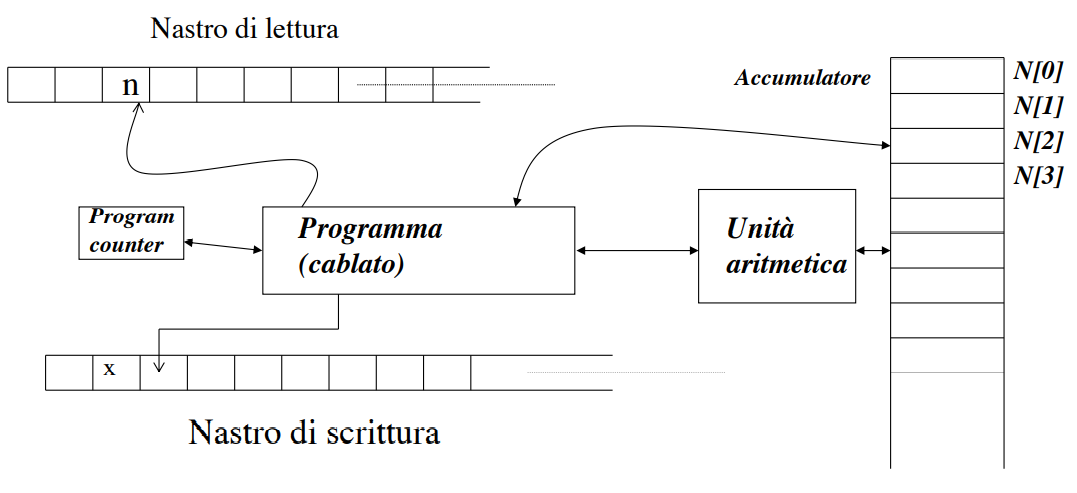
\includegraphics[width=\textwidth]{RAM.png}
  \end{figure}

  Sia i nastri che la memoria sono composti da un numero illimitato di celle, ma al contrario dei nastri di ingresso e uscita che si possono accedere in maniera sequenziale, la memoria è indirizzata e si può accedere a una sua cella attraverso un numero intero \(i>0\) che indica l'indirizzo di tale cella di memoria. La cella 0 della memoria è un registro speciale, detto accumulatore, che si utilizza per contenere il valore di uno dei due operandi delle operazioni aritmetiche binarie che la macchina può effettuare. Un generico porgramma eseguibile dalla macchina RAM è composto da istruzioni riportate nella tabella \ref{tabella istruzioni RAM}.

  \begin{table}[!h] 
    \caption{istruzioni macchina RAM}
    \vspace*{10pt}
    
    \centering
    \begin{tabular}{l l | l} \label{tabella istruzioni RAM}
      ISTRUZIONE & & SEMANTICA\\
      \hline
      LOAD= & \(x\) & M[0] \(\leftarrow x\)\\
      LOAD & \(x\)  & M[0] \(\leftarrow\) M[\(x\)]\\
      LOAD* & \(x\) & M[0] \(\leftarrow\) M[M[\(x\)]]\\
      STORE & \(x\) & M[\(x\)] \(\leftarrow\) M[0]\\
      STORE* & \(x\) & M[M[\(x\)]] \(\leftarrow\) M[0]\\
      ADD= & \(x\) & M[0] \(\leftarrow\) M[0] + \(x\)\\
      ADD  & \(x\)& M[0] \(\leftarrow\) M[0]+ M[\(x\)]\\
      ADD* & \(x\)& M[0] \(\leftarrow\) M[0] + M[M[\(x\)]]\\
      SUB= & \(x\)& M[0] \(\leftarrow\) M[0] - \(x\)\\
      SUB & \(x\)& M[0] \(\leftarrow\) M[0] - M[\(x\)]\\
      SUB* & \(x\)& M[0] \(\leftarrow\) M[0] - M[M[\(x\)]]\\
      MULT= & \(x\)& M[0] \(\leftarrow\) M[0] * \(x\)\\
      MULT & \(x\)& M[0] \(\leftarrow\) M[0] * M[\(x\)]\\
      MULT* & \(x\)& M[0] \(\leftarrow\) M[0] * M[M[0]]\\
      DIV= & \(x\)& M[0] \(\leftarrow\) M[0] \(\backslash\) \(x\) \\
      DIV & \(x\)& M[0] \(\leftarrow\) M[0] \(\backslash\) M[\(x\)]\\
      DIV* & \(x\)& M[0] \(\leftarrow\) M[0] \(\backslash\) M[M[\(x\)]]\\
      READ & \(x\)& M[x] \(\leftarrow\) input\\
      READ* & \(x\)& M[M[x]] \(\leftarrow\) input\\
      WRITE= & \(x\)& stampa \(x\)\\
      WRITE & \(x\)& stampa M[\(x\)]\\
      WRITE* & \(x\)& stampa M[M[\(x\)]]\\
      JUMP & \(label\)& PC \(\leftarrow\) \(label\) \\
      JGZ & \(label\)& PC \(\leftarrow\) \(label\) if M[0] \(>\) 0\\
      JLZ & \(label\)& PC \(\leftarrow\) \(label\) if M[0] \(<\) 0 \\
      JZ & \(label\)& PC \(\leftarrow\) \(label\) if M[0] = 0\\
      HALT & & terminazione\\
    \end{tabular}
  \end{table}

  Una volta introdotte tutte le istruzioni eseguibili dalla macchina RAM, è possibile ora studiarne la complessità temporale, come fatto per le TM a \(k\)-nastri. A differenza delle TM, nelle macchine RAM l'esecuzione delle diverse operazioni dipende dagli operandi necessari per eseguire tale operazione. Diventa quindi necessario analizzare tutte le istruzioni e definire il tempo richiesto per ciascuna di esse e la quantità di memoria allocata. Queste quantità possono essere calcolate secondo due criteri, ovvero tramite il criterio del costo costante e tramite il criterio del costo logaritmico. Il primo si basa sull'assunzione che l'esecuzione di ciascuna istruzione richieda un'unità di tempo e che ciascuna allocazione in memoria richieda un'unità di spazio (stessa assunzione fatta per le TM). 
  
  Si è appena affermato però che nella macchina RAM le istruzioni hanno diversa natura e manipolano dati di diversa dimensione: risulta, dunque, evidente che tale criterio è poco affine alla realtà. Per tener conto della differente velocità di esecuzione e della differente quantità di memoria allocata da ciascuna istruzione, si introduce il secondo criterio (del costo logaritmico), basato sulla supposizione che il tempo richiesto per eseguire un'istruzione sia proporzionale alla lunghezza degli operandi dell'istruzione considerata. Poichè gli operandi sono rappresentati in memoria in codice binario, un generico operando di valore \(v\) è rappresentato da \(\lfloor log_2(|v|+1)\rfloor\). 
  
  Dunque, è possibile definire la funzione \(l(i) = if\;i\neq 0\;then\;\lfloor log_2(|v|+1)\rfloor\;else\;1\) tramite cui calcolare la complessità temporale logaritmica di ciascuna istruzione precedentemente analizzata nella tabella \ref{tabella istruzioni RAM}. Alla stessa maniera, è possibile calcolare i costi relativi allo spazio, introducendo la variabile \(m\) definita come l'indirizzo più alto della cella di memoria a cui si fa accesso durante l'esecuzione del programma, e la variabile \(M_i\) che rappresenta il valore assoluto più grande immagazzianto in M[i] durante l'esecuzione. La complessità spaziale logaritmica si definisce quindi con la seguente formula:

  \(\displaystyle \sum_{i=0}^m{l(M_i)}\)\\
  Di seguito sono riportati i costi logaritmici delle istruzioni RAM:

  \begin{table}[!htb] \label{tabella costi logaritmici}
    \caption{costi logaritmici delle istruzioni macchina RAM}
    \vspace*{10pt}
    
    \centering
    \begin{tabular}{l l | l}
      ISTRUZIONE & & COSTO LOGARITMICO\\
      \hline
      LOAD= & \(x\) & \(l(x)\)\\
      LOAD & \(x\)  & \(l(x) + l(M[x])\) \\
      LOAD* & \(x\) & \(l(x) + l(M[x]) + l(M[M[x]])\)\\
      STORE & \(x\) & \(l(M[0]) + l(x)\)\\
      STORE* & \(x\) & \(l(M[0]) + l(x) + l(M[x])\)\\
      ADD= & \(x\) & \(l(M[0]) + l(x)\)\\
      ADD  & \(x\)& \(l(M[0]) + l(x) + l(M[x])\)\\
      ADD* & \(x\)& \(l(M[0]) + l(x) + l(M[x]) + l(M[M[x]])\)\\
      & & SUB, MULT, DIV definite come ADD.\\
      READ & \(x\)& \(l(input) + l(x)\)\\
      READ* & \(x\)& \(l(input) + l(x) + l(M[x])\)\\
      WRITE= & \(x\)& \(l(x)\)\\
      WRITE & \(x\)& \(l(x) + l(M[x])\)\\
      WRITE* & \(x\)& \(l(x) + l(M[x]) + l(M[M[x]])\)\\
      JUMP & \(label\)& 1 \\
      JGZ & \(label\)& \(l(M[0])\)\\
      JLZ & \(label\)& \(l(M[0])\) \\
      JZ & \(label\)& \(l(M[0])\)\\
      HALT & & 1\\
    \end{tabular}
  \end{table}
  
  Dunque, il criterio del costo costante si può applicare solo in situazioni in cui si prevede che ogni valore che comparirà durante l'esecuzione del programma occupi esattamente una cella di memoria, altrimenti si deve necessariamente applicare il criterio del costo logaritmico, che porta ad un calcolo più preciso della complessità.
  

  \section{Correlazione temporale fra TM e RAM}
  Una volta analizzato il comportamento della macchina RAM, è possibile studiarne la correlazione con le TM. Nello specifico, è possibile simulare una TM deterministica a \(k\) nastri attraverso una macchina RAM, nel seguente modo: innanzitutto, si considera la memoria della RAM come suddivisa in blocchi, tutti di dimensione \(k\), ad eccezione del blocco 0, che ha dimensione \(k+1\), in quanto memorizza lo stato della TM e le posizioni delle \(k\) testine. I successivi blocchi vengono impiegati per contenere i valori contenuti nelle successive posizioni di ciascuno dei \(k\) nastri di memoria della TM. Dunque, il valore rappresentato nella \(i\)-esima cella del \(j\)-esimo nastro della TM è contenuto nella locazione \(c+k\cdot j+i\) in cui \(c\) è una costante opportuna della memoria della macchina RAM. 
  Inoltre, per accedere al valore presente sotto la testina di lettura di un determinato nastro è prima necessario eseguire un accesso diretto al blocco 0, per poter trovare la posizione del nastro stesso. Poi, per eseguire la funzione di transizione \(\delta(q,i,s_1,...,s_k)\) e la funzione di uscita \(\eta(q,i,s_1,...,s_k)\), si richiedono un numero prefissato di accessi in memoria per ottenere \(q,i,s_1,...,s_n\), necessari per l'esecuzione di tali funzioni.

  Tutto ciò conduce al seguente teorema:

  \begin{theorem}
    Una TM multinastro con complessità temporale \(T_M\) può essere simulata da una macchina RAM con complessità temporale \(T_R = \Theta( T_M)\), secondo il criterio di costo uniforme, oppure \(T_R = \Theta( T_M \cdot log( T_M))\), secondo il criterio di costo logaritmico. 
  \end{theorem}

  Ovviamente è possibile anche simulare una macchina RAM tramite una macchina di Turing, ma tale costruzione è molto più complessa e richiede un'analisi approfondita. Si enuncia quindi solo il seguente teorema:

  \begin{theorem}
    Sia L il linguaggio riconosciuto da una macchina RAM di complessità temporale \({T}_R\) secondo il criterio del costo logaritmico. Se il programma RAM non utilizza le istruzioni \(MULT\) e \(DIV\), allora L può essere riconosciuto da un'opportuna TM multinastro, in un tempo \({T}_M=\Theta({T}_R^2)\). 
  \end{theorem}

  Si può quindi osservare come il legame tra \({T}_M\) e \({T}_R\) sia di tipo polinomiale, implicazione molto importante perchè suggerisce quale sia la classe di problemi trattabili nella pratica.